\subsection{Ejercicio 15}
\graphicspath{ {img/15} }

\paragraph{Apartado a)} Dentro de las opciones disponibles en el plan gratuito de ProtonVPN podemos destacar \textbf{Quick connect}, que nos permite conectarnos a una VPN escogida automáticamente, en vez de seleccionar manualmente el país/servidor al que conectarnos (en este plan solamente tendremos disponibles conexiones a Japón, Holanda, Polonia, Rumanía y Estados Unidos). Además, contamos con algunas opciones extra en el apartado \texttt{Settings}, como por ejemplo:

\begin{tcolorbox}[
    colback=orange!5!white,
    colframe=orange!75!black,
    title=Opciones relevantes en ProtonVPN
]
\begin{itemize}
    \item \textbf{Kill Switch:} Nos desconecta automáticamente si perdemos la conexión a la VPN.
    \item \textbf{Protocol:} Nos permite cambiar el protocolo de conexión. Podemos elegir entre WireGuard o las dos opciones de OpenVPN: TCP o UDP.
    \item \textbf{IPv6:} Permite filtrar el tráfico que utilice IPv6 a través de la VPN, lo cual aumenta la compatibilidad con redes que utilicen este protocolo.
    \item \textbf{Otras opciones:} También contamos con una opción de cambio de plan además de opciones sobre la aplicación en local, como el iniciarla minimizada o seleccionar nuestras conexiones preferidas como prioritarias.
\end{itemize}
\end{tcolorbox}


\paragraph{Apartado b)} Antes de activar ProtonVPN, miramos las direcciones públicas y privadas de nuestra máquina, además de comprobar nuestra calidad de conexión con el CESGA, mediante RedIRIS.

Como podemos ver en la figura \ref{fig:IPs}, en un principio nuestra IP privada es \\\texttt{192.168.1.141} y la pública \texttt{93.156.217.17}.
Además, nuestra conexión con el CESGA es de \SI{10}{ms} de ping, \SI{2.82}{ms} de jitter, \SI{292}{Mbps} de descarga y \SI{210}{Mbps} de subida.

Estos parámetros son normales dada la distancia que tenemos con el CESGA y que nos estamos conectando directamente.

\begin{figure}[H]
    \centering
    \begin{subfigure}{.5\textwidth}
        \centering
        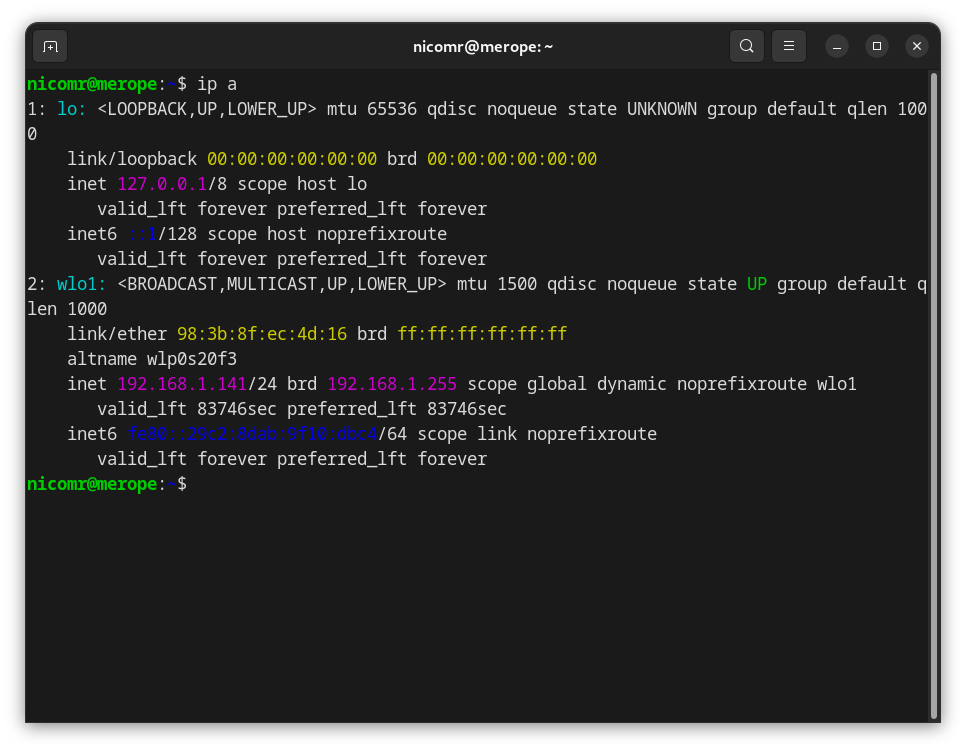
\includegraphics[width=\linewidth]{IP-Privada.png}
        \caption{Dirección IP Privada}
    \end{subfigure}%
    \begin{subfigure}{.5\textwidth}
        \centering
        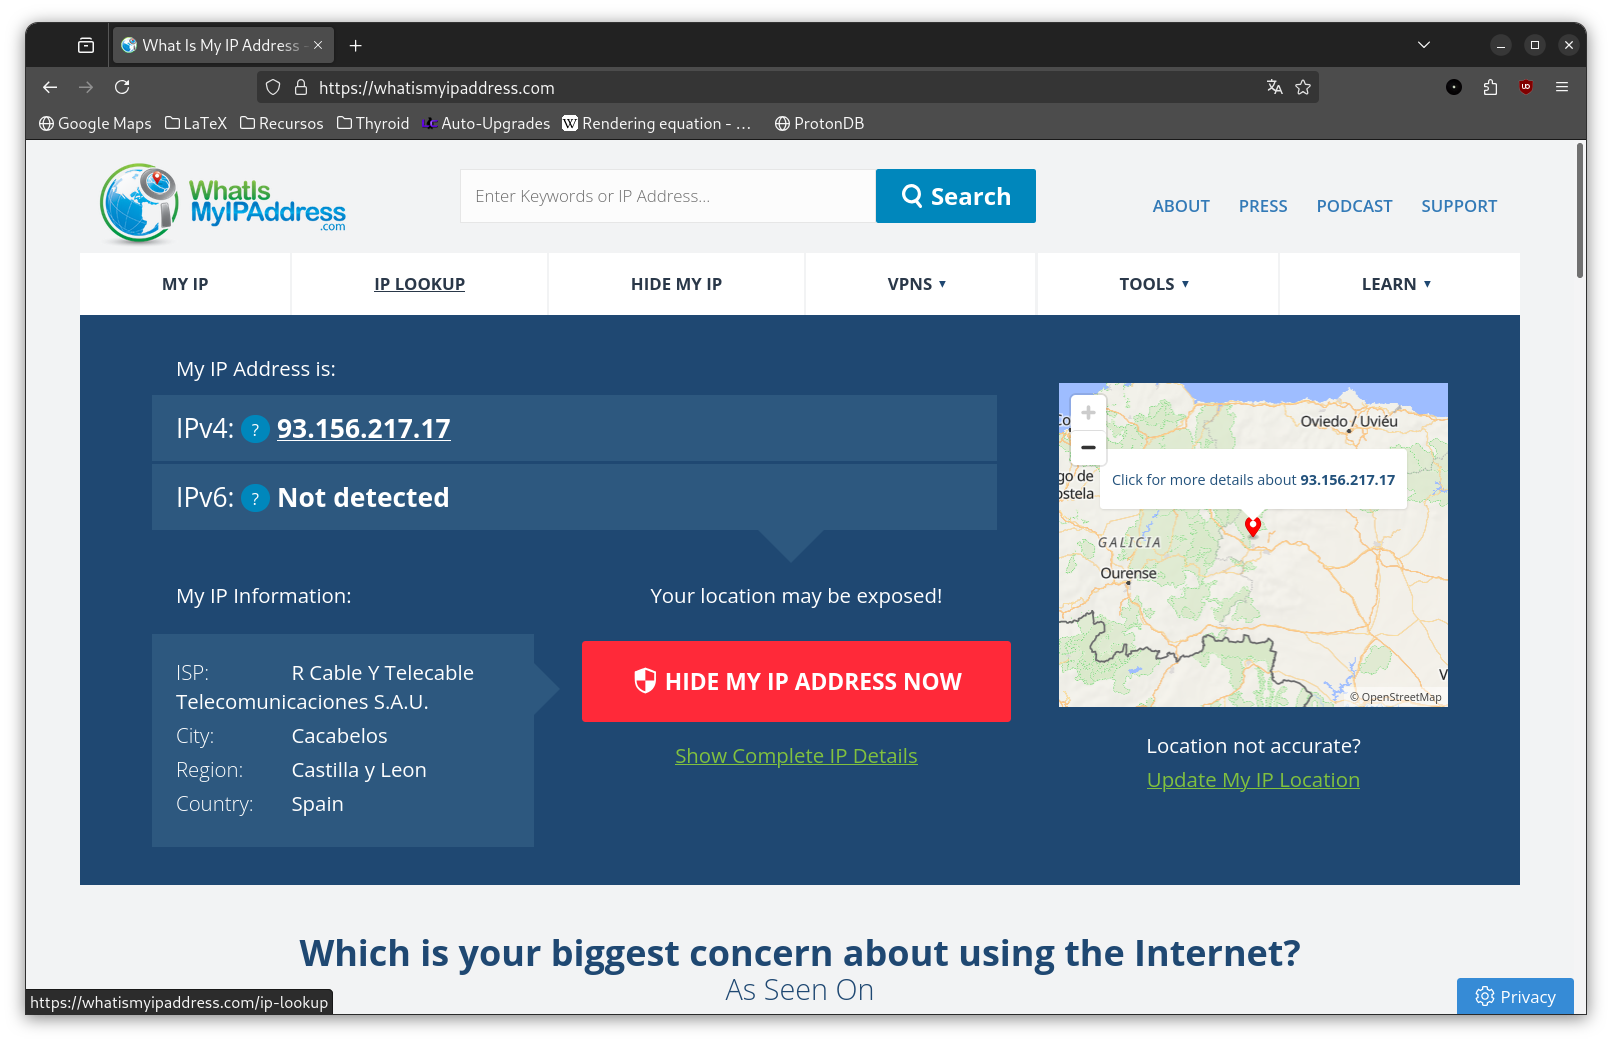
\includegraphics[width=\linewidth]{IP-Publica.png}
        \caption{Dirección IP Pública}
    \end{subfigure}
    \caption{Direcciones IP sin ProtonVPN}
    \label{fig:IPs}
\end{figure}


\begin{figure}[H]
    \centering
    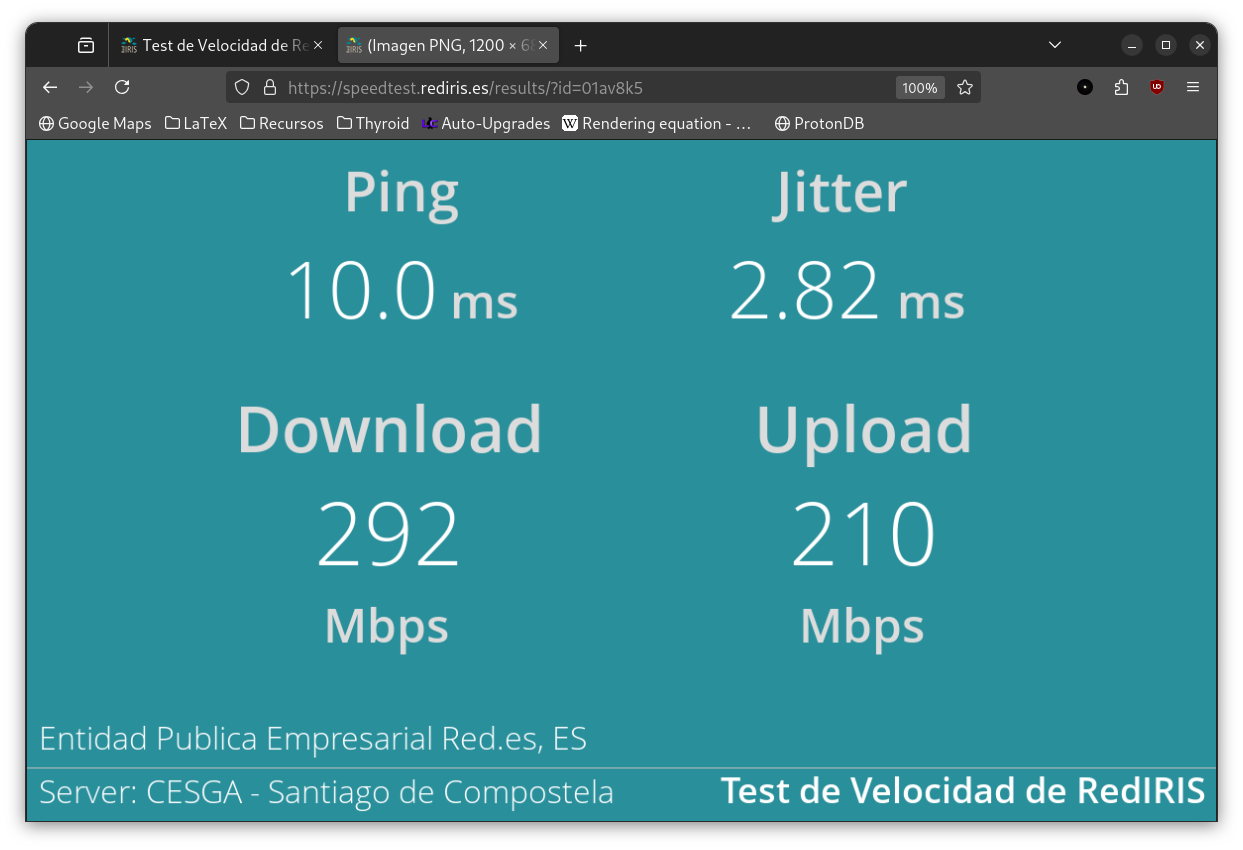
\includegraphics[width=\linewidth]{CalidadConexion.png}
    \caption{Calidad de la conexión sin ProtonVPN}
    \label{fig:Calidad-Conexión}
\end{figure}


Ahora, activamos ProtonVPN con Quick Connect, por ejemplo. En nuestro caso nos conectó a un servidor de Holanda.

En la figura \ref{fig:IPs-Holanda} podemos ver el resultado. Se observa que han aparecido dos interfaces de red nuevas, una para IPv4 y otra para IPv6, respectivamente. Esto seguramente sea debido a que activamos la opción IPv6 en los ajustes de ProtonVPN.

En cuanto a las direcciones IP, nuestra dirección privada a utilizar será \texttt{10.98.0.40}, mientras que la pública ha cambiado a \texttt{185.177.126.134}.

Si comprobamos nuestra calidad de red como en la figura \ref{fig:Calidad-Conexión-Holanda} vemos que han aumentado el ping y el jitter, mientras que las velocidades de subida y descarga han disminuído, como es de esperar.

\begin{figure}[H]
    \centering
    \begin{subfigure}{.5\textwidth}
        \centering
        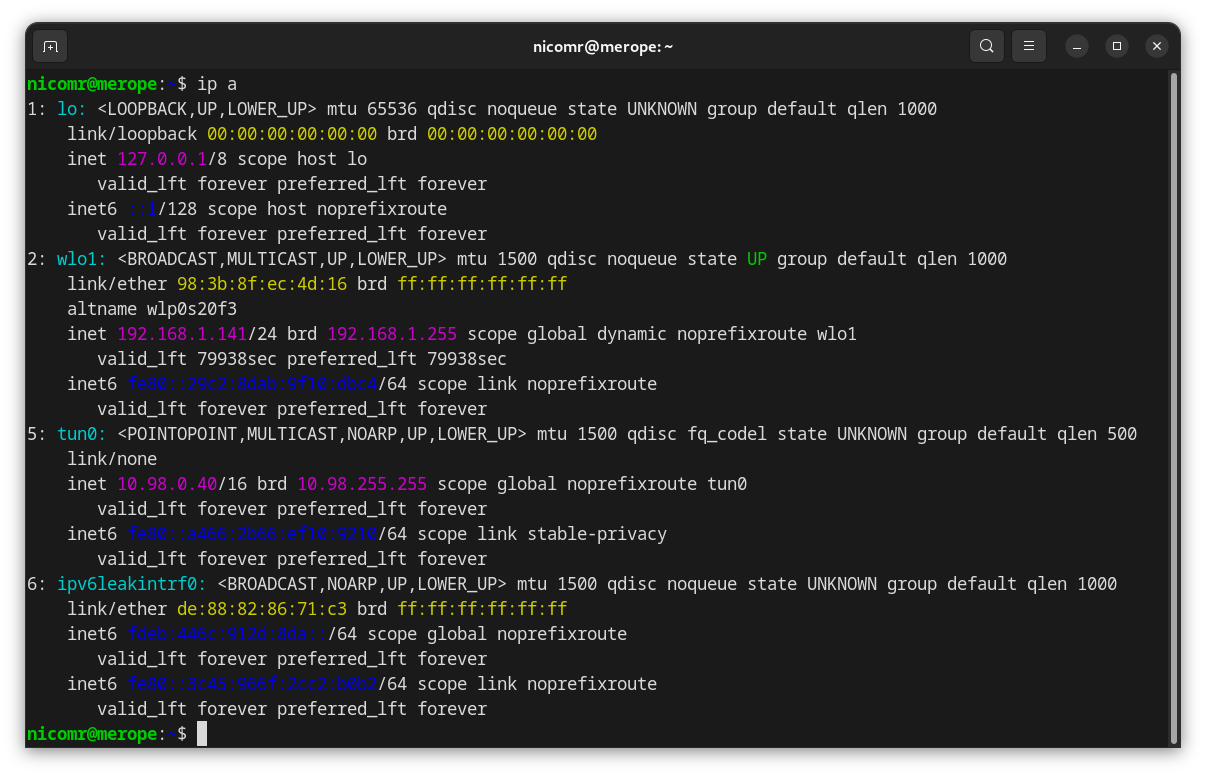
\includegraphics[width=\linewidth]{IP-Privada-Holanda.png}
        \caption{Dirección IP Privada}
    \end{subfigure}%
    \begin{subfigure}{.5\textwidth}
        \centering
        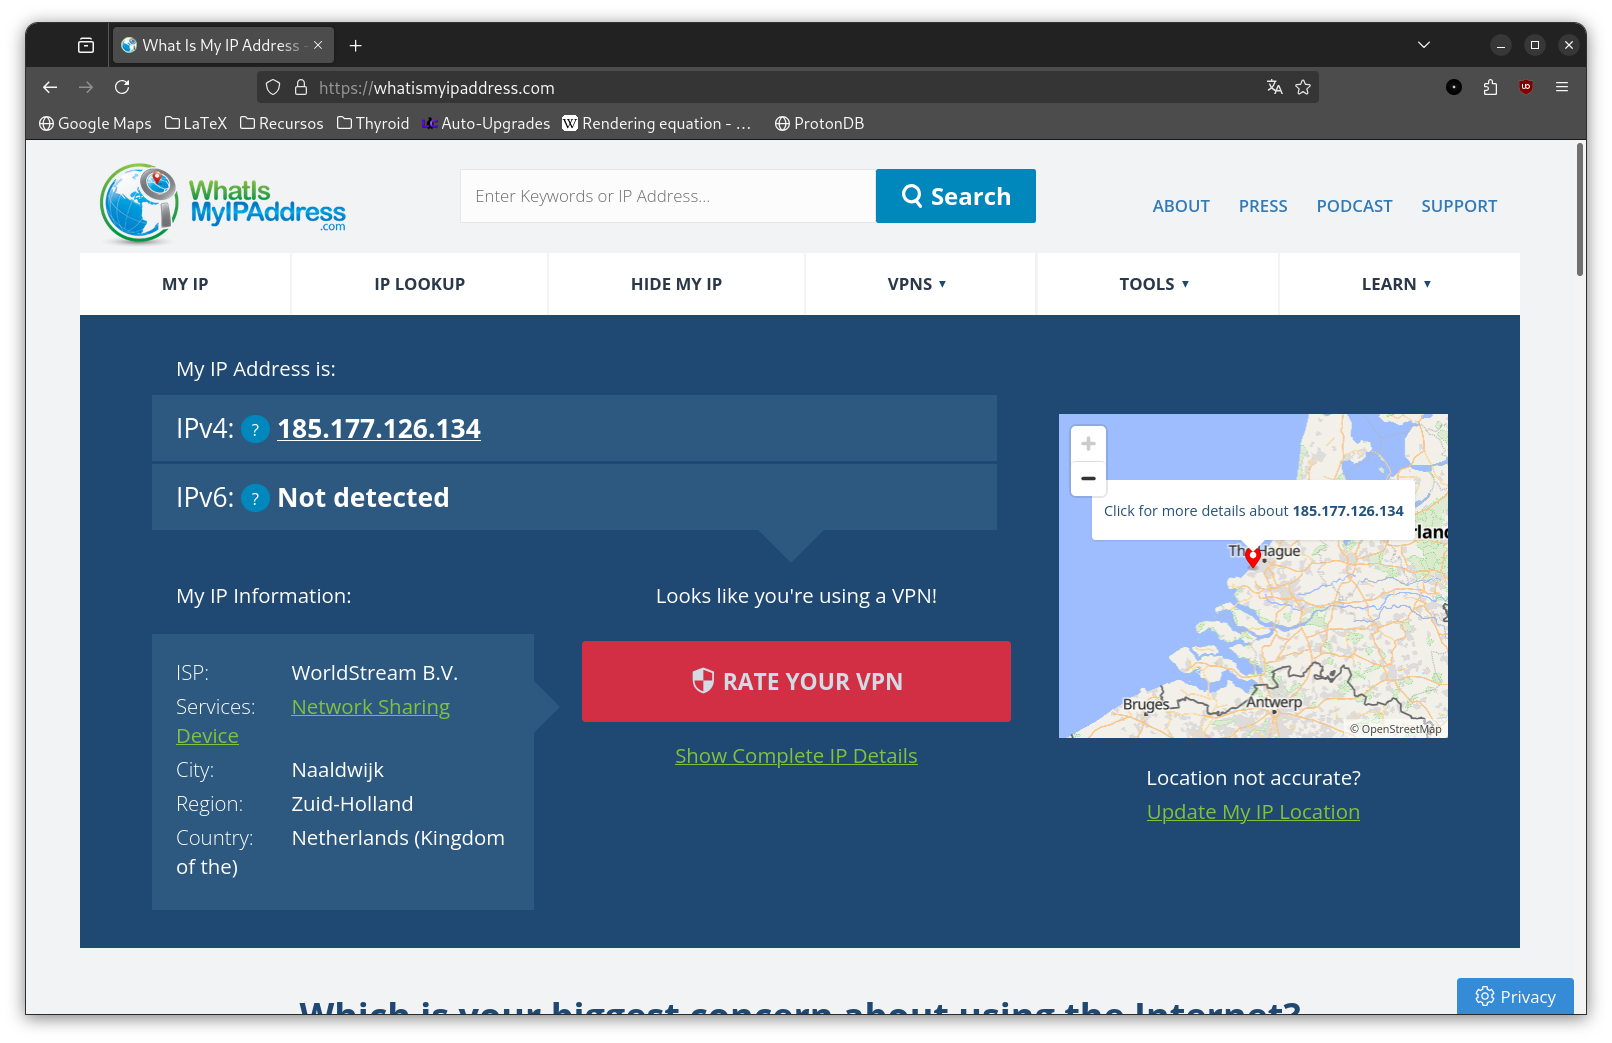
\includegraphics[width=\linewidth]{IP-Publica-Holanda.png}
        \caption{Dirección IP Pública}
    \end{subfigure}
    \caption{Direcciones IP desde Holanda}
    \label{fig:IPs-Holanda}
\end{figure}

\begin{figure}[H]
    \centering
    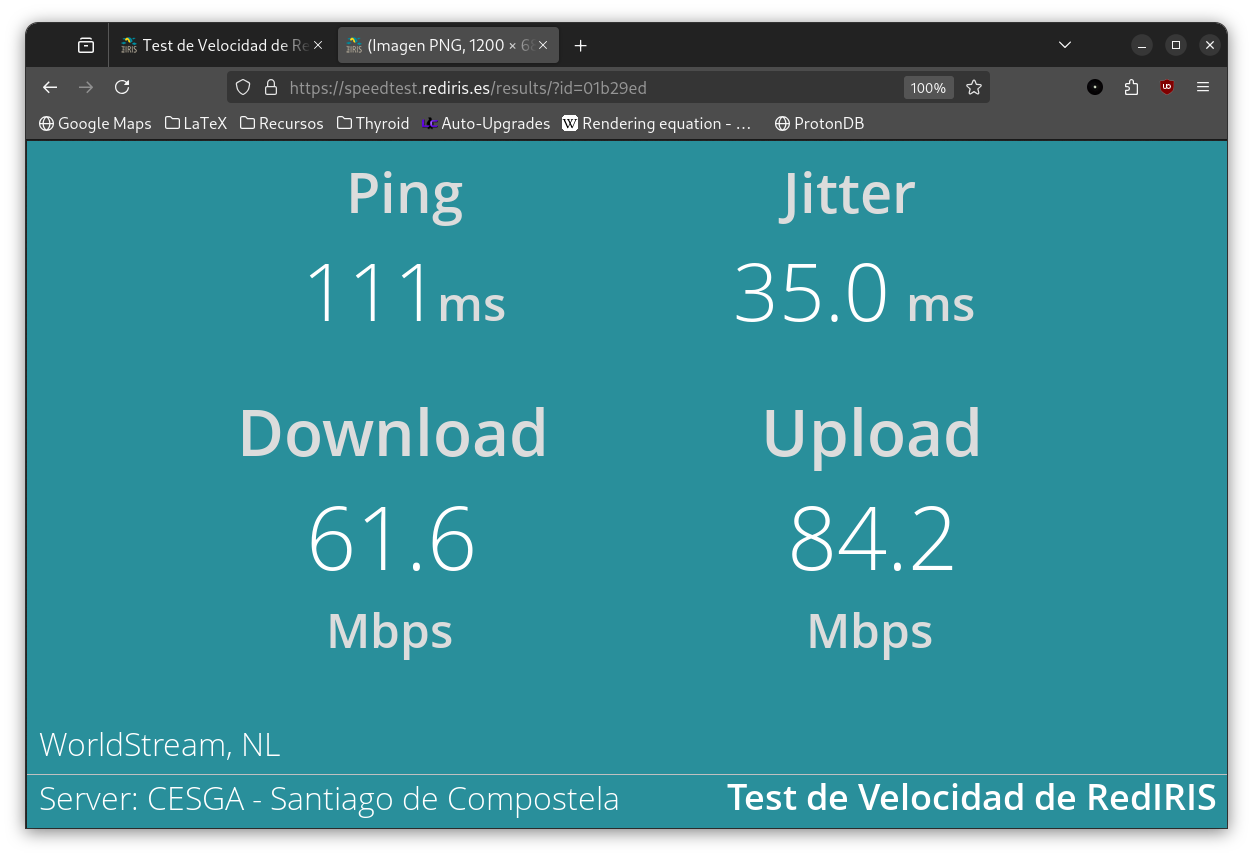
\includegraphics[width=\linewidth]{CalidadConexion-Holanda.png}
    \caption{Calidad de la conexión desde Holanda}
    \label{fig:Calidad-Conexión-Holanda}
\end{figure}


A continuación repetiremos el proceso otras dos veces más (tres en total) cambiando de servidor. La primera con un servidor en Rumanía y la segunda con un servidor en Japón.
Los resultados se muestran desde la figura \ref{fig:IPs-Rumania} a la figura \ref{fig:Calidad-Conexión-Japon}.

\begin{figure}[H]
    \centering
    \begin{subfigure}{.5\textwidth}
        \centering
        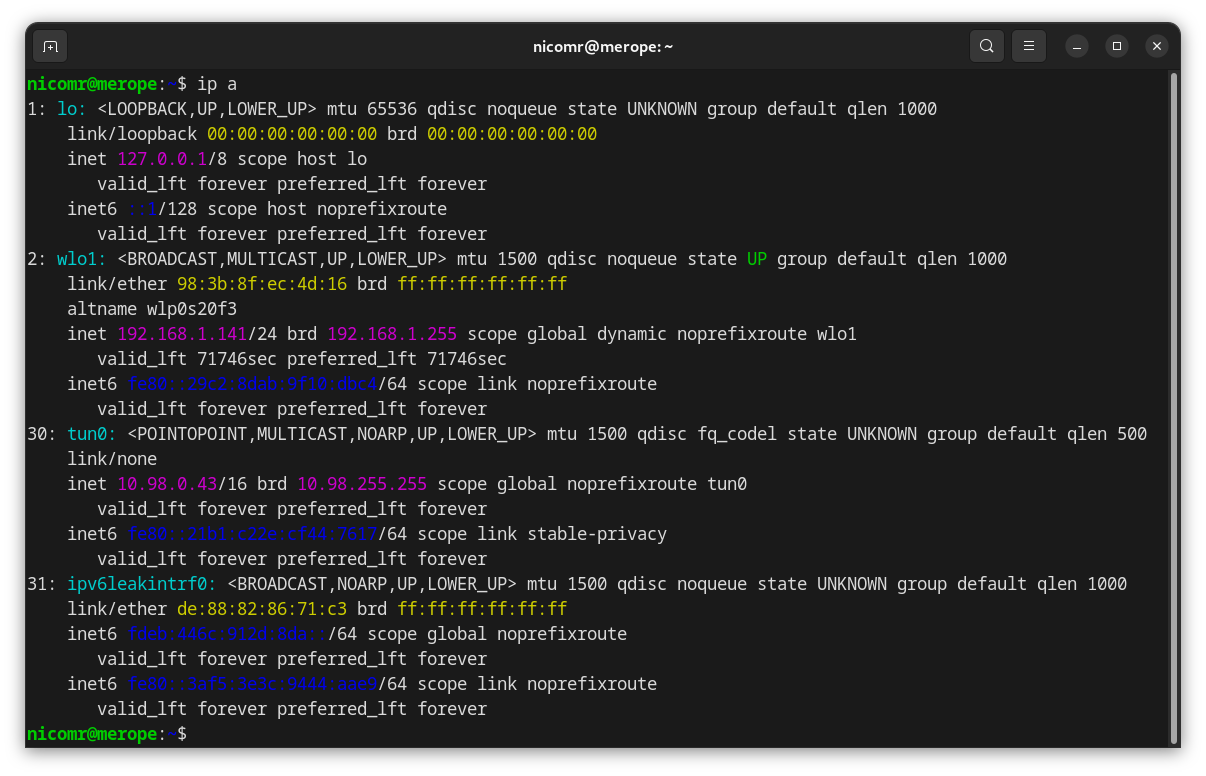
\includegraphics[width=\linewidth]{IP-Privada-Rumania.png}
        \caption{Dirección IP Privada}
    \end{subfigure}%
    \begin{subfigure}{.5\textwidth}
        \centering
        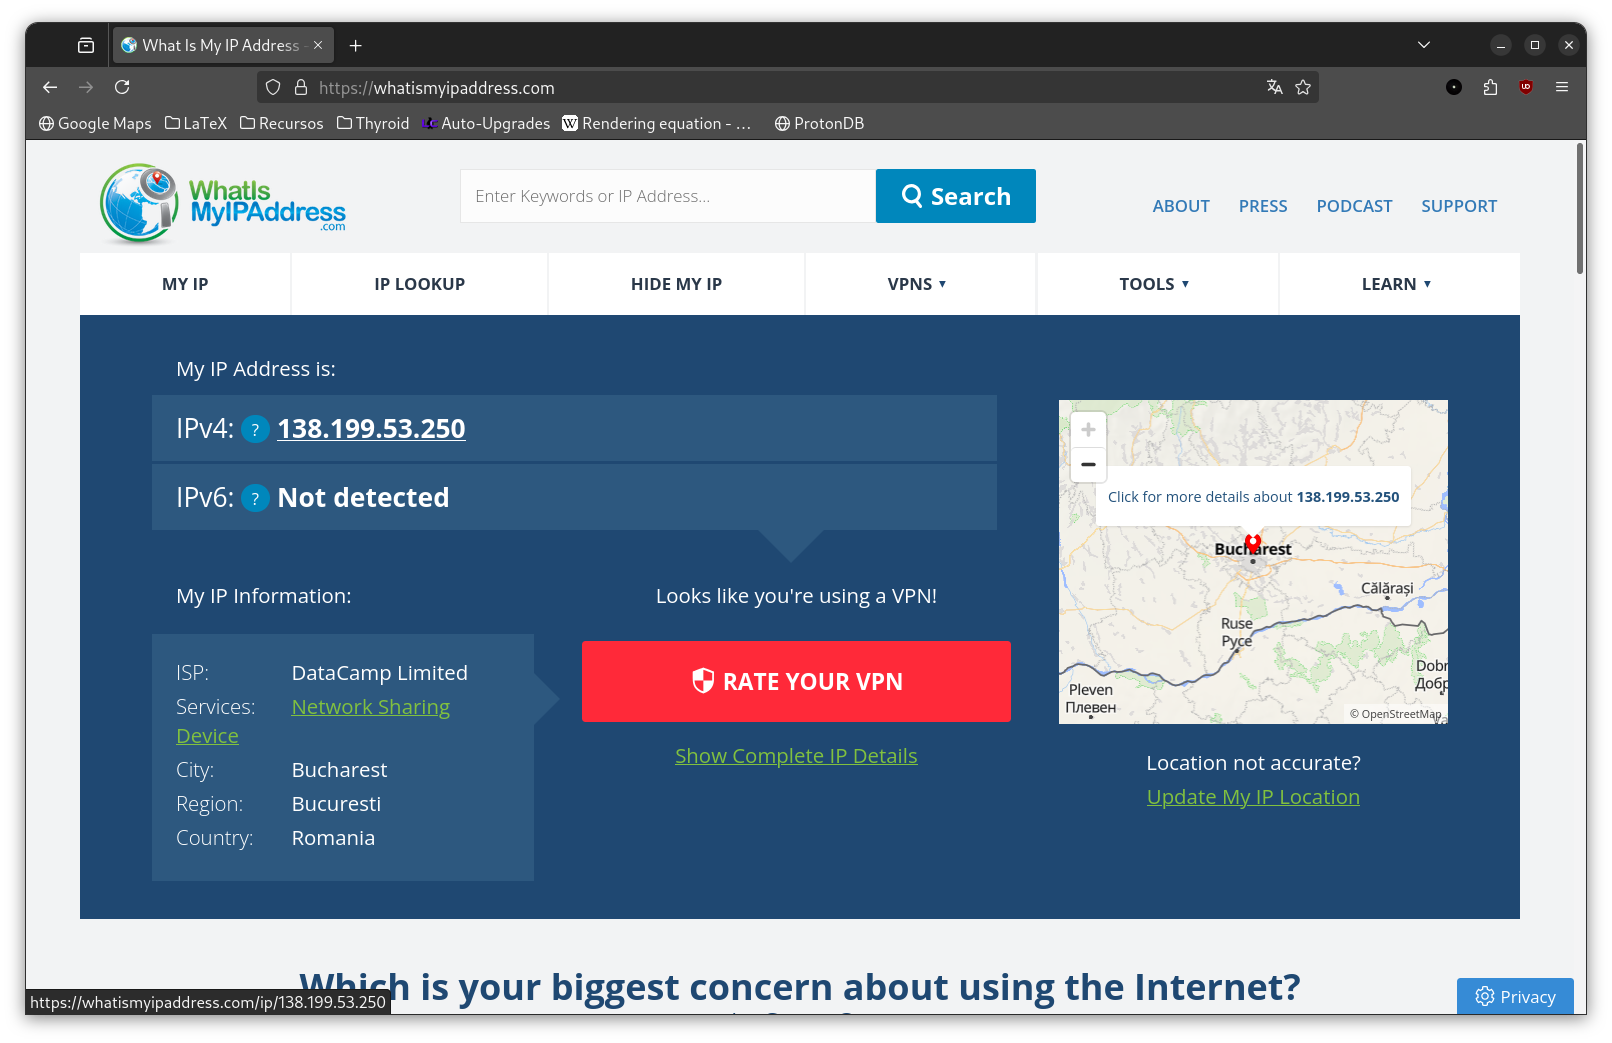
\includegraphics[width=\linewidth]{IP-Publica-Rumania.png}
        \caption{Dirección IP Pública}
    \end{subfigure}
    \caption{Direcciones IP desde Rumania}
    \label{fig:IPs-Rumania}
\end{figure}

\begin{figure}[H]
    \centering
    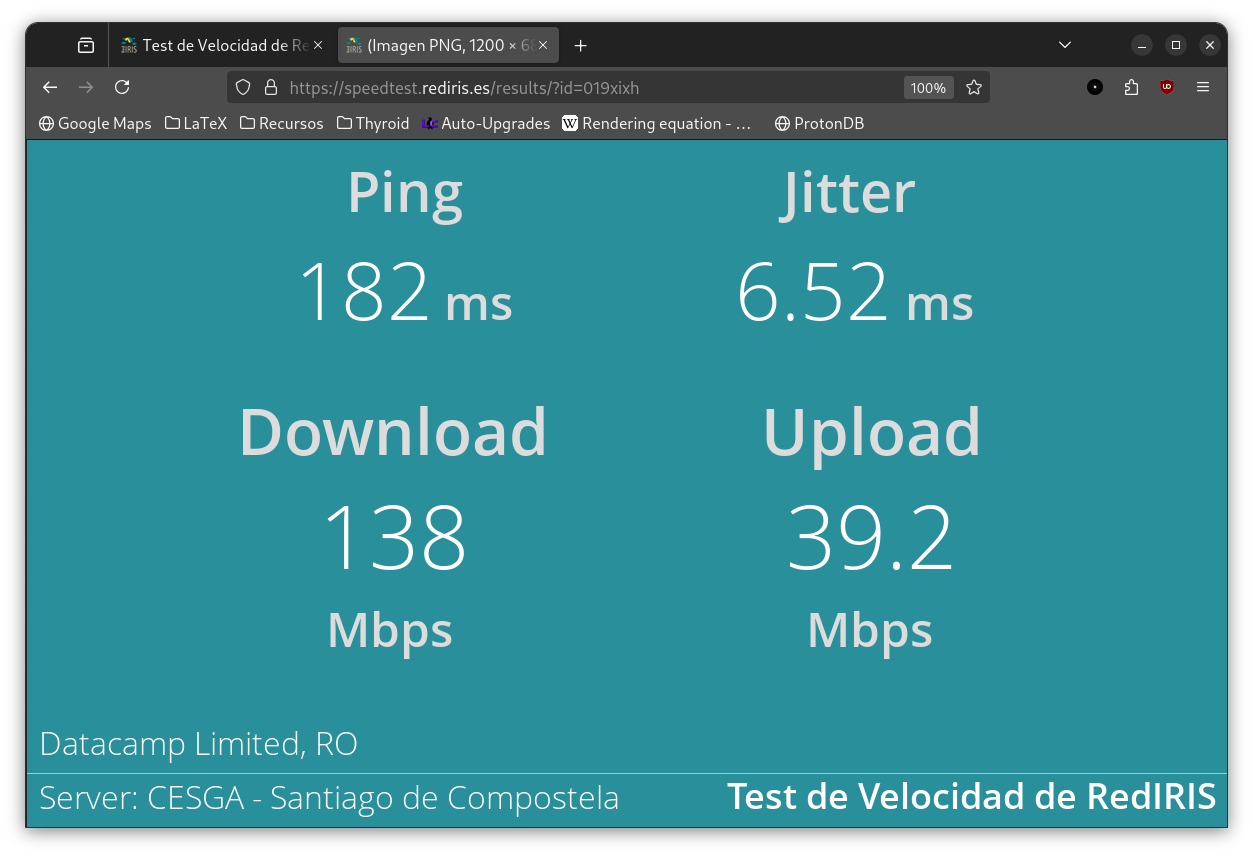
\includegraphics[width=\linewidth]{CalidadConexion-Rumania.png}
    \caption{Calidad de la conexión desde Rumania}
    \label{fig:Calidad-Conexión-Rumania}
\end{figure}


\begin{figure}[H]
    \centering
    \begin{subfigure}{.5\textwidth}
        \centering
        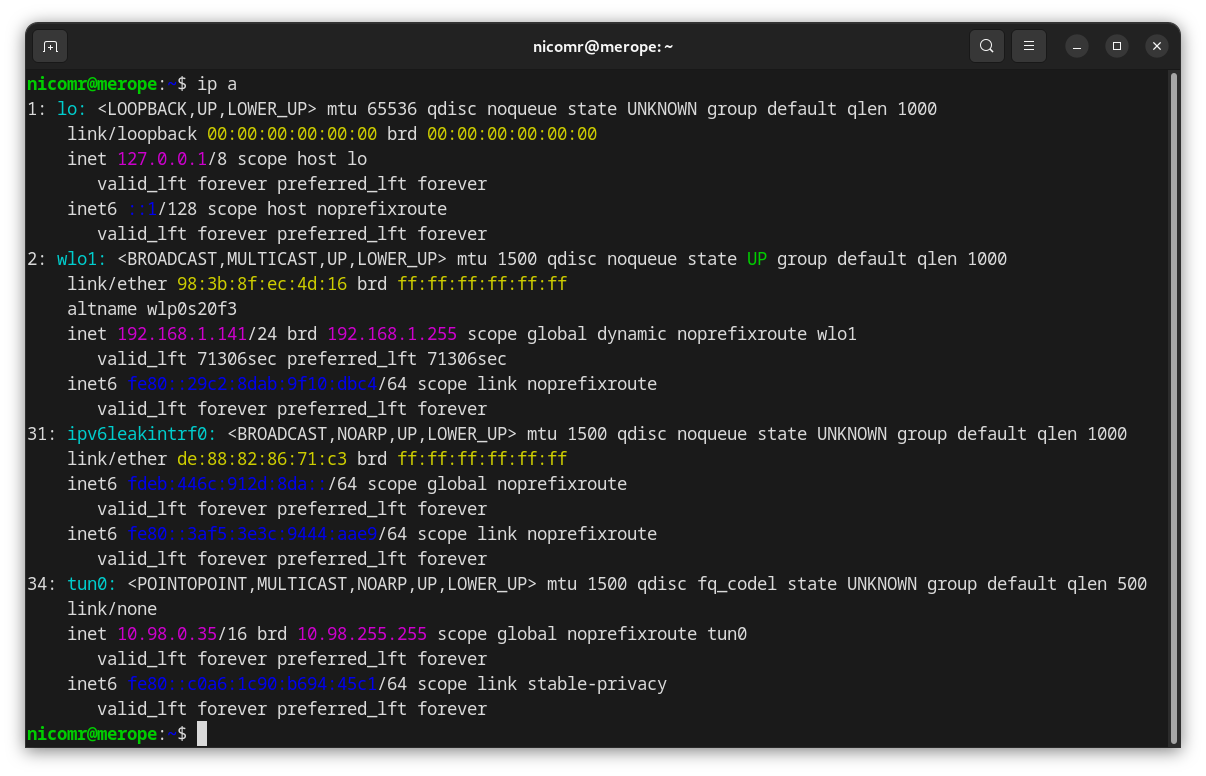
\includegraphics[width=\linewidth]{IP-Privada-Japon.png}
        \caption{Dirección IP Privada}
    \end{subfigure}%
    \begin{subfigure}{.5\textwidth}
        \centering
        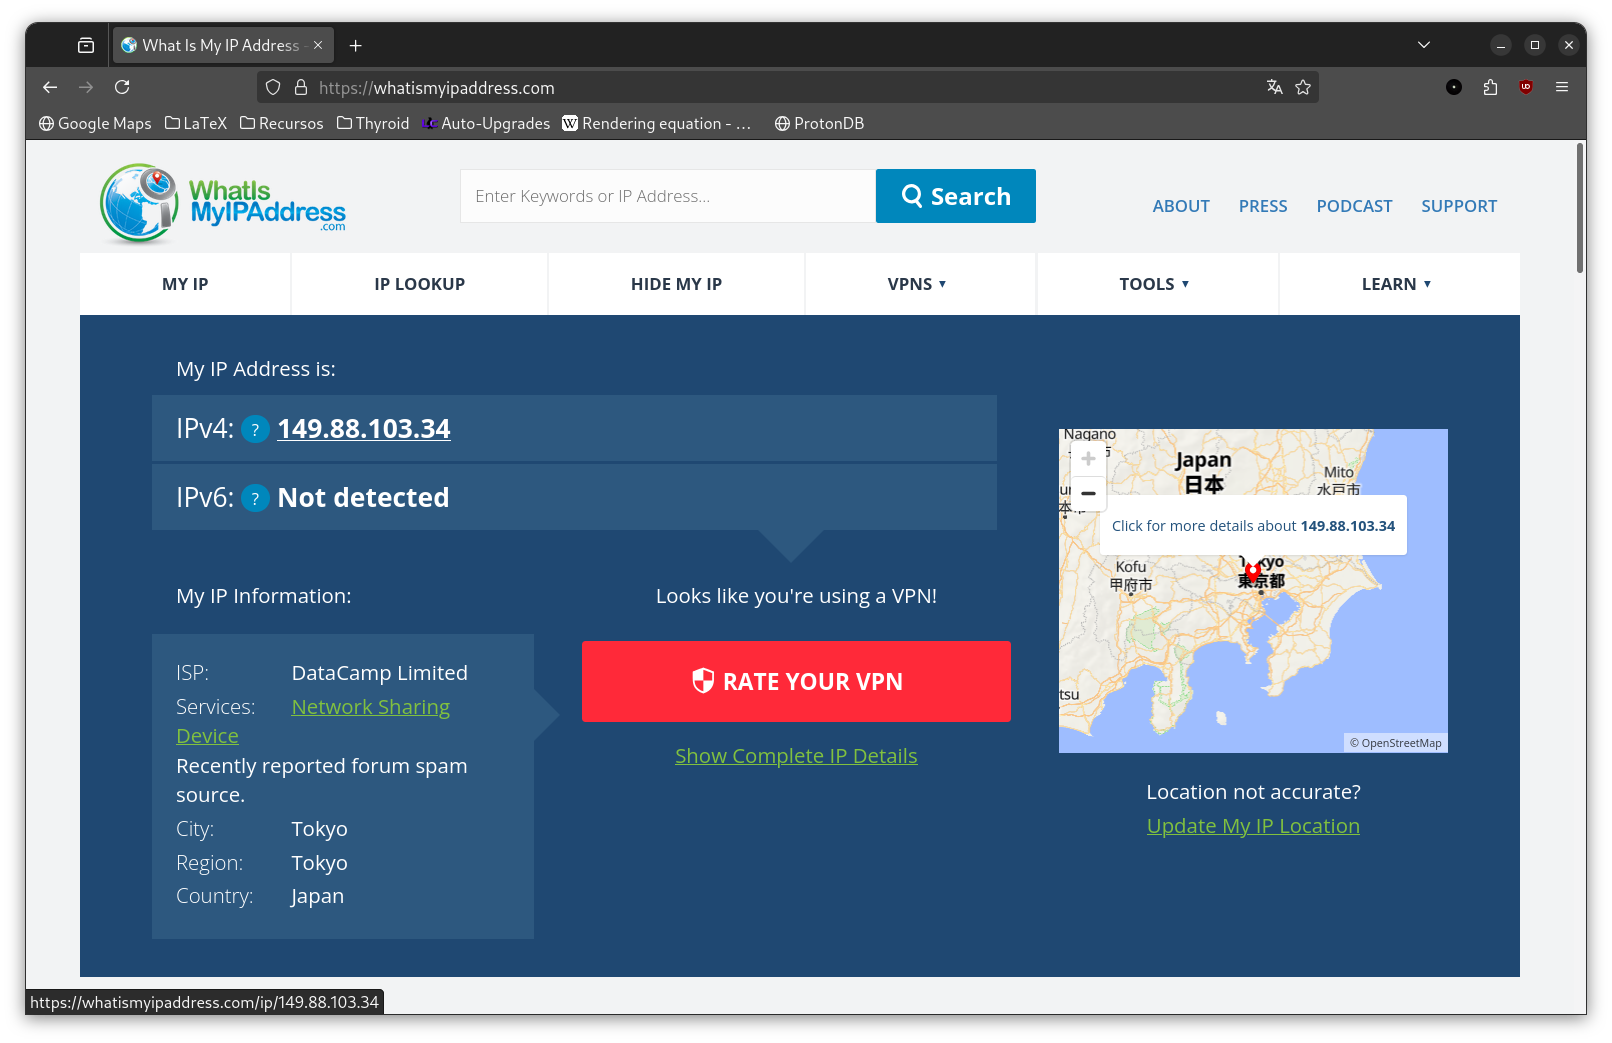
\includegraphics[width=\linewidth]{IP-Publica-Japon.png}
        \caption{Dirección IP Pública}
    \end{subfigure}
    \caption{Direcciones IP desde Japon}
    \label{fig:IPs-Japon}
\end{figure}

\begin{figure}[H]
    \centering
    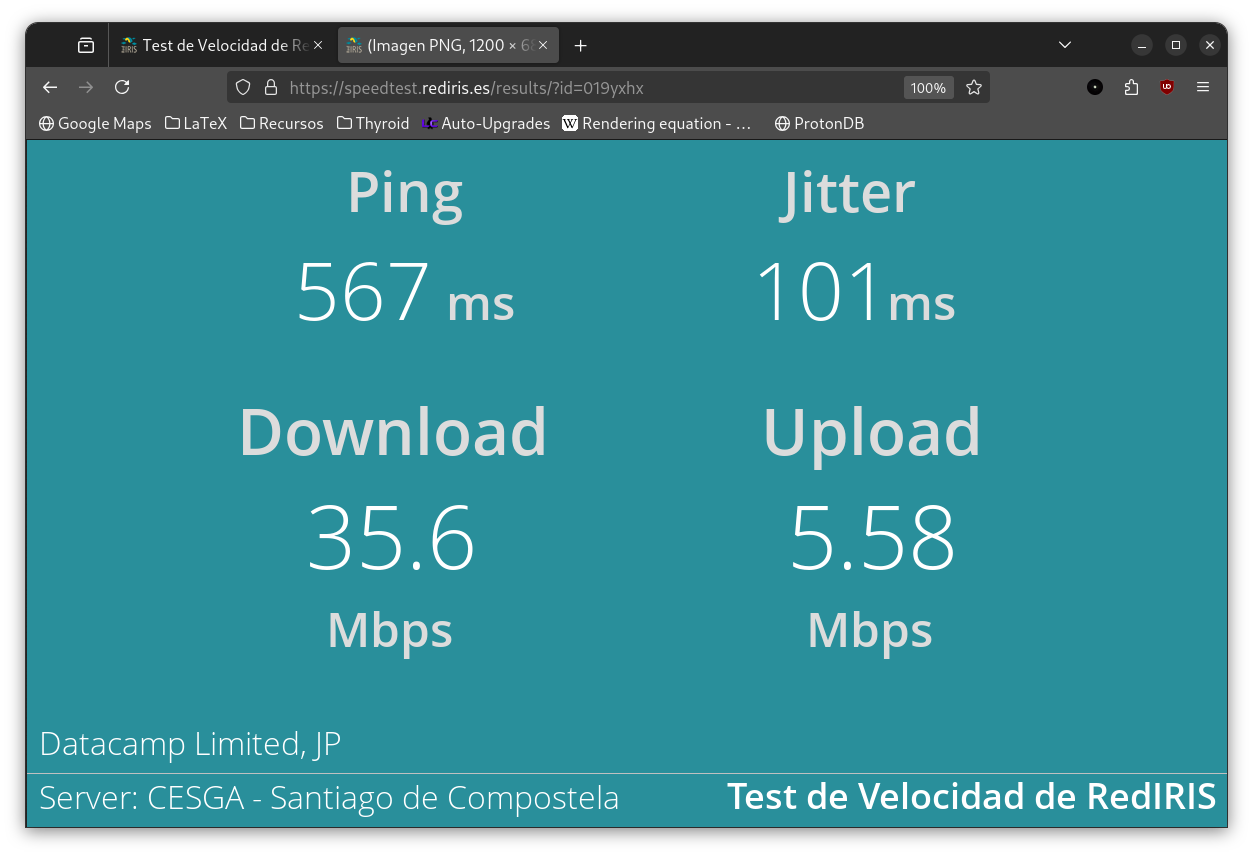
\includegraphics[width=\linewidth]{CalidadConexion-Japon.png}
    \caption{Calidad de la conexión desde Japon}
    \label{fig:Calidad-Conexión-Japon}
\end{figure}
